\documentclass[12pt]{beamer}

\usetheme{CambridgeUS}
\usecolortheme{beaver}
\setbeamertemplate{navigation symbols}{}

\usepackage[utf8]{inputenc}
%\usepackage[croatian]{babel}

\date{}

\hypersetup{draft}

\title{Očitavanje senzorskih podataka korištenjem računala Raspberry Pi 3}
\author{Leonard Volarić Horvat\\ Mentori: \\ Nenad Katanić, mag. ing.\\
Doc. dr. sc. Boris Milašinović}

\institute[FER]{Sveučilište u Zagrebu\\Fakultet elektrotehnike i računarstva}

\begin{document}

{
	\setbeamertemplate{headline}[]
	\setbeamertemplate{footline}{}
	\begin{frame}
		\maketitle
	\end{frame}
}

\begin{frame}
	Sadržaj:
	\tableofcontents
\end{frame}

\section{Raspberry Pi}
\begin{frame}
\frametitle{Raspberry Pi}
	\begin{itemize}
		\item Vrlo popularno računalo malih dimenzija
		\item Odlike:
		\begin{itemize}
			\item Visoka fleksibilnost
			\item Dobre performanse
			\item Niska cijena
		\end{itemize}
		\item Vrlo raširena i pristupačna zajednica korisnika
	\end{itemize}
\end{frame}

\subsection{Sklopovlje}
\begin{frame}
	\frametitle{Raspberry Pi 3 - sklopovlje}
	\begin{columns}[T]
	    \begin{column}{.5\textwidth}
		\begin{figure}[h]
			\begin{minipage}{\textwidth}
				\centering
				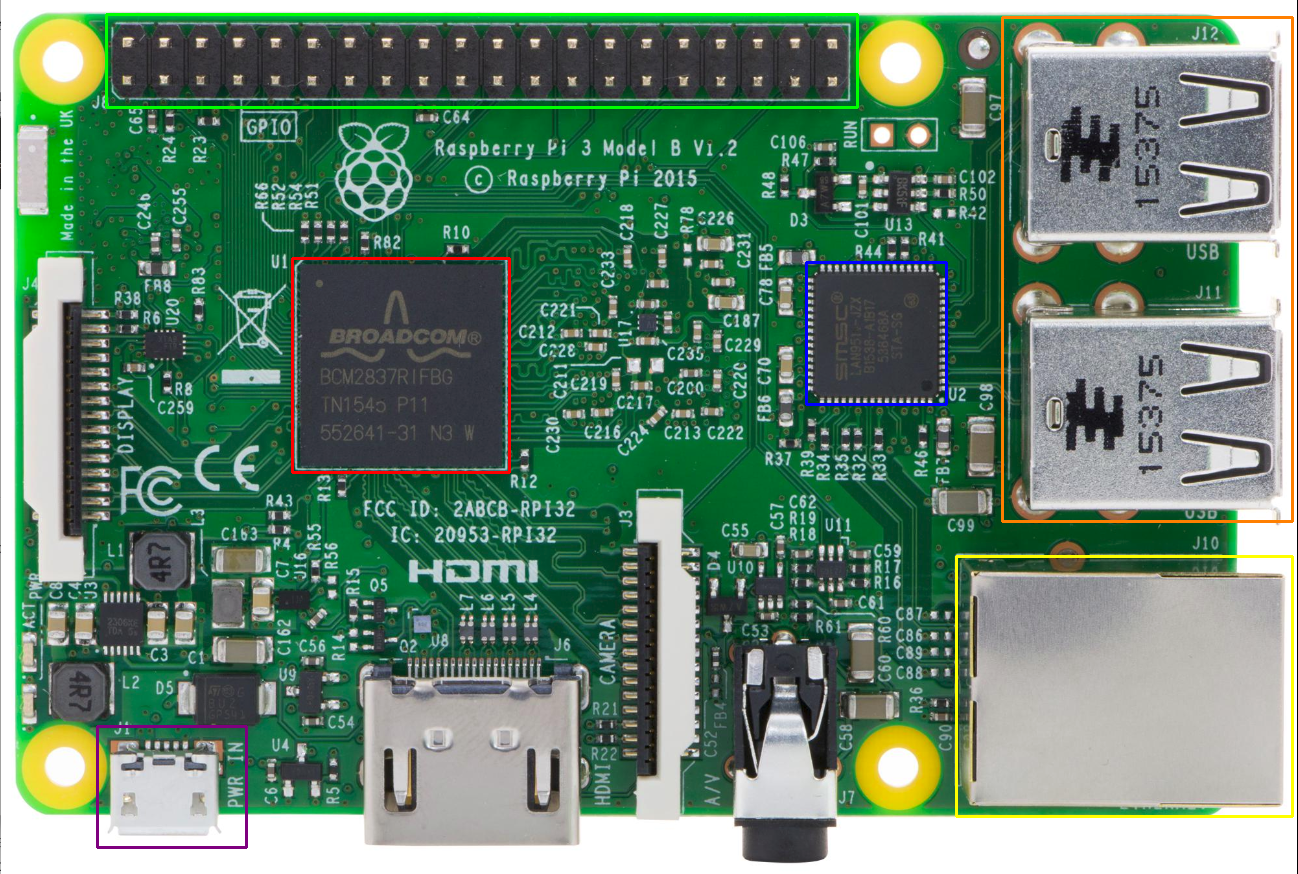
\includegraphics[width=\linewidth]{slike/rpi3_color.png}
			\end{minipage}
		\end{figure}
		Broadcom BCM2837
			\begin{itemize}
				\item CPU - četverojezgreni ARMv8, 1.2GHz
				\item GPU - VideoCore IV, 400MHz
			\end{itemize}
		\end{column}

		\begin{column}{.5\textwidth}
			\begin{itemize}
				\item Podrška za WiFi i Bluetooth
				\item Glavni ulazno-izlazni priključci:
				\begin{itemize}
					\item 4 USB 2.0 priključka
					\item Ethernet priključak
					\item microUSB priključak za napajanje
					\item sučelje sa 40 GPIO pinova
					\item ulaz za microSD karticu
				\end{itemize}
			\end{itemize}
		\end{column}
	\end{columns}
\end{frame}

\subsection{Programska podrška}
\begin{frame}
	\frametitle{Raspberry Pi - programska podrška}
	\begin{figure}[h]
			\begin{minipage}{0.2\textwidth}
				\centering
				
\includegraphics[width=\linewidth]{slike/raspbian-logo.png}
			\end{minipage}
		\end{figure}
	Raspbian - najpopularniji OS za RPi
	\begin{itemize}
		\item Distribucija Linuxa bazirana na Debianu
		\item Pokreće se s microSD kartice
		\item Besplatan i otvoren
		\item OS optimiziran za RPi sklopovlje
	\end{itemize}
\end{frame}

\subsection{Primjeri korištenja}
\begin{frame}
	\frametitle{Raspberry Pi - primjeri korištenja}
	Pametna brava
	\begin{itemize}
		\item Autorizacija pomoću lozinke, kartice, prepoznavanja lica...
		\item Praćenje autoriziranih ulaza u prostor
	\end{itemize}
	\vfill
	VPN i WiFi pristupna točka
	\begin{itemize}
		\item Ostvarivanje kućnog VPN-a
		\item Stvaranje \textit{ad hoc} WiFi pristupne točke
	\end{itemize}
\end{frame}

\section{Senzori}
\subsection{Akcelerometar - Adafruit LIS3DH}
\begin{frame}
	\frametitle{Akcelerometar - Adafruit LIS3DH}
	\begin{columns}[T]
	    \begin{column}{.5\textwidth}
		\begin{figure}[h]
			\begin{minipage}{\textwidth}
				\centering
				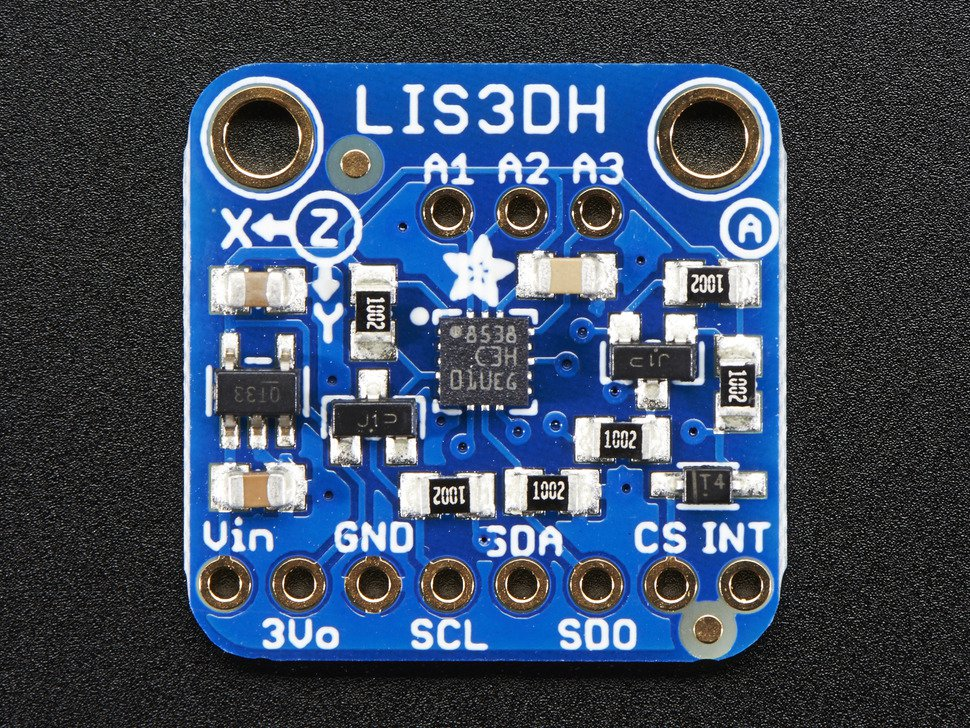
\includegraphics[width=\linewidth]{slike/lis3dh.jpg}
			\end{minipage}
		\end{figure}
		Akcelerometar tvrtke Adafruit
		\end{column}

		\begin{column}{.5\textwidth}
			\begin{itemize}
				\item Mjerenje na 3 osi
				\item 10-bitna preciznost
				\item Podrška za I$^2$C i SPI protokole
				\item Vrlo mala potrošnja
				\item Niska cijena
			\end{itemize}
			\begin{itemize}
				\item Prekidni pin
				\item Ulazi za ADC
			\end{itemize}
		\end{column}
	\end{columns}
\end{frame}

\subsection{Mikrofon - Adafruit MAX4466}
\begin{frame}
	\frametitle{Mikrofon - Adafruit MAX4466}
	\begin{columns}[T]
	    \begin{column}{.5\textwidth}
		\begin{figure}[h]
			\begin{minipage}{\textwidth}
				\centering
				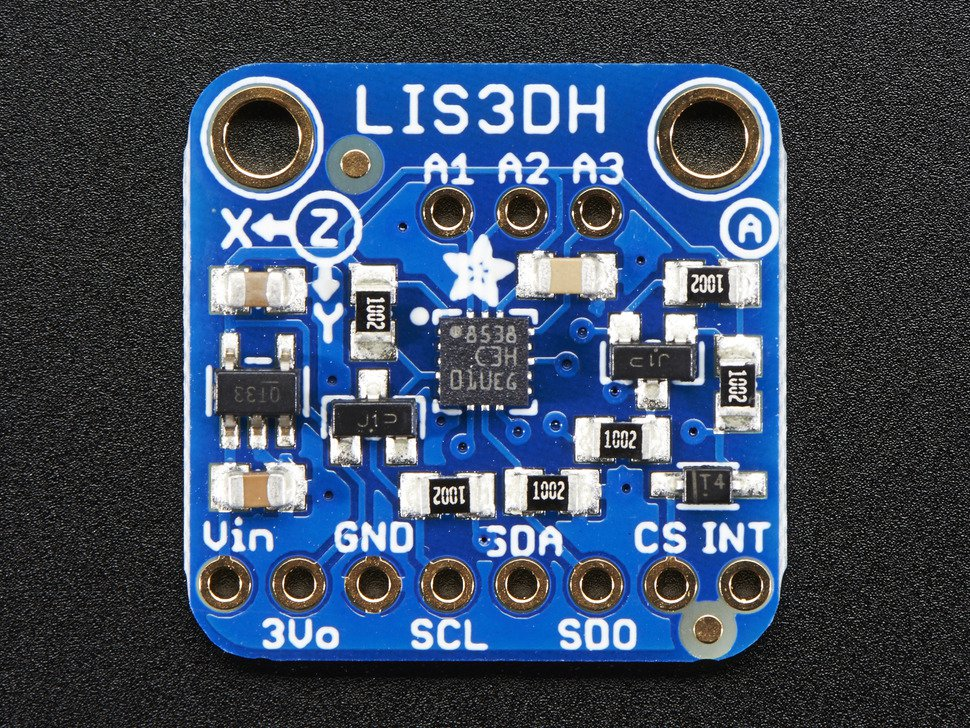
\includegraphics[width=\linewidth]{slike/lis3dh.jpg}
			\end{minipage}
		\end{figure}
		Elektretski mikrofon tvrtke Adafruit
		\end{column}

		\begin{column}{.5\textwidth}
			Dva glavna funkcijska dijela:
			\begin{itemize}
				\item Elektretski mikrofon (20Hz - 20kHz)
				\item Operacijsko pojačalo Maxim MAX4466
			\end{itemize}
			\begin{itemize}
				\item Sklopovski upravljivo pojačanje
				\item Samo analogni izlaz $\longrightarrow$ nužan ADC sklop
			\end{itemize}
		\end{column}
	\end{columns}
\end{frame}

\section{Dostupni programski okviri}
\begin{frame}
	\frametitle{Dostupni programski okviri}
	GPIO komunikacija u Pythonu:
	\begin{itemize}
		\item Adafruitova biblioteka
	\end{itemize}

	Komunikacija GPIO i LIS3DH:
	\begin{itemize}
		\item Neslužbena biblioteka \texttt{python-lis3dh}
	\end{itemize}

	Komunikacija GPIO i MAX4466:
	\begin{itemize}
		\item Analogni izlazi $\longrightarrow$ ADC $\longrightarrow$ GPIO čitanje ADC izlaz
	\end{itemize}
\end{frame}

\subsection{Primjer mjerenja}
\begin{frame}
	\frametitle{Opis mjerenja}
	Korišten LIS3DH \\
	Mjerenja:
	\begin{enumerate}
		\item Senzor pričvršćen za stol:
		\begin{itemize}
			\item Kucanje
			\item Udaranje
		\end{itemize}
		\item Senzor pričvršćen za bas gitaru
			\begin{itemize}
			\item Odsviran ton A (55Hz)
		\end{itemize}
	\end{enumerate}
\end{frame}

\end{document}